\documentclass[12pt,letterpaper]{article}
\usepackage[margin=1in]{geometry}
\usepackage{graphicx}
\usepackage{amsmath}

\usepackage[hidelinks]{hyperref}
\hypersetup{
    colorlinks=true,
    linkcolor=blue,
    filecolor=magenta,      
    urlcolor=cyan,
}

\hyphenation{Model-Sim}

\begin{document}

\title{LEG Processor for Education\\\Large{System Documentation}
}
\author{Contact: \\Max Waugaman (mwaugaman@hmc.edu) \\Sam Dietrich (sdietrich@hmc.edu)}
\date{Last Modified \today}
\maketitle
\thispagestyle{empty}
\pagebreak
\setcounter{page}{1}
\pagebreak

\tableofcontents
\pagebreak

\section{Getting Started}
\subsection{Installation} \label{sec:install}
LEG processor development begins by downloading the code base to your local machine or a shared class drive.
The code is small enough for each user to have a local copy for development and testing.
After cloning the LEG repository, only a few off the shelf programs are required to get the processor running.
Complete instructions are presented here for Linux systems, but most functionality is available on Windows.

Several programs must be installed to use the full LEG debugger. 
However, only the LEG repository must be downloaded if you are simply interested in examining the source files.

\begin{enumerate}
\item Install git and clone the LEG git repository from \url{https://github.com/MWaug/LEG}. 
The next installation steps only need to be one once per machine you are installing the LEG debugging system on.

\item Install packages required for the debugging tools. We needed to install the packages listed below to run the debugging framework on our 64-bit system, but your requirements may vary.
They can be installed using your package manager.

\begin{tabular}{|l|l|}
\hline 
\textbf{Package} & \textbf{Needed for} \\\hline
g++ & QEMU, GDB, debug\_lockstep \\\hline
libtool & QEMU \\\hline
zlib1g-dev & QEMU \\\hline
libglib2.0-dev & QEMU \\\hline
libpixman-1-dev & QEMU \\\hline
libfdt-dev & QEMU \\\hline
libpython2.7:i386 & GDB \\\hline
lib32ncurses5 & GDB \\\hline
libxft2:i386 & ModelSim \\\hline
libxext6:i386 & ModelSim \\\hline
python (2.7)& debug\_lockstep \\\hline
\end{tabular}

\item Choose a path on your system to install the required debugging tools. 
Be sure that this path is readable by everyone who will be using LEG on your system.
Throughout the examples in this guide, the path will be \texttt{/legproj/}

\item Install the free Starter Edition of ModelSim from \url{http://dl.altera.com} or any version of ModelSim you may already have purchased. 
Note that in Starter Edition performance may be reduced and some minor features such as checkpoints will be unavailable. 
LEG has been tested on ModelSim version SE 10.3d. 

\item Install GDB and GCC for bare metal ARM systems from \url{https://launchpad.net/gcc-arm-embedded} and untar into your LEG installation directory. 
For example, \\\texttt{/legproj/gcc-arm-none-eabi-5\_3-2016q1}.\\
Instructions for this are provided in the readme available at the same website.

\item The QEMU system emulator must be downloaded and installed from source. 
\textbf{NOTE}: The patches required for LEG will possibly break every QEMU system except \\\texttt{qemu-system-arm}. 
To keep this guide simple the default QEMU build process is used. 
You can safely remove systems other than \texttt{arm-softmmu}.
	\begin{enumerate}
	\item Clone the QEMU source into your central LEG directory: \\\texttt{git clone git://git.qemu-project.org/qemu.git}
	\item From this QEMU directory, run the following commands: \\\texttt{git checkout -b leg-additions v2.4.0 \\ git am leg/repo/path/qemu\_patches/*.patch}\\
	where \texttt{leg/repo/path} is the path to your LEG git repository, not the folder for debugging tools.
	These commands will apply the custom LEG addons to v2.4.0 of QEMU.
	\item In the QEMU directory run \\\texttt{./configure \\ sudo make -j20}\\ to build QEMU.
	\end{enumerate}
	
\item The Linux executable for LEG debugging can be found in \\\texttt{leg/repo/path/kernel}. 
LEG uses \href{https://www.busybox.net}{BusyBox} 1.23.1, which can be compiled from source using the instructions in \texttt{kernel-setup-info}.
Unless you wish to rebuild Linux, the only action necessary is to untar the file \texttt{system.tar.gz}:
\\In \texttt{kernel/}, run \texttt{tar -zxvf system.tar.gz}
\end{enumerate}

Now all software necessary to run the LEG testing tools should be installed, but some components must still be configured.
These short steps are described in the next section.

\subsection{Configuration}\label{sec:cfg}

Certain variables must be set to provide LEG access to the programs it needs for testing.
These steps will get you there.

\begin{enumerate}
\item Add the ModelSim tools (vsim) to your system path.
These are most likely found in the \texttt{modelsim\_ase/linuxaloem} directory of your ModelSim installation.
For example, using the path name and ModelSim version referenced in the previous section, we would edit our \texttt{.bashrc} file and add the following line: \\\texttt{export PATH="/legproj/altera/15.1/modelsim\_ase/linuxaloem:\$PATH"}

\item Navigate to \texttt{leg/repo/path/debug\_lockstep} and modify the file \texttt{config\-uration.py} with the following. 
Examples are included in the file.
	\begin{enumerate}
		\item set \texttt{qemu\_path} to the path to \texttt{qemu\_system\_arm}
		\item set \texttt{gdb\_path} to the path to \texttt{arm-none-eabi-gdb-py}
		\item set \texttt{hasVopt} to 0 if you are using ModelSim SE, or 1 if you have a version of ModelSim with vopt.
		\item set \texttt{linux\_path} to the path of the Linux executable. This should already be set unless you compiled your own version.
	\end{enumerate}
	
\item For waveform debugging it is useful to have another ModelSim project that can quickly load saved processor state from a certain instruction.
See Section \ref{sec:MSdebug} for information on debugging in ModelSim using this setup.
	\begin{enumerate}
		\item Create a folder \texttt{MSdebug} in your LEG repository path and create a new ModelSim project named \texttt{msdebug} in it.
		If you use different names you will need to edit \texttt{qemuDumpRestore\_MS.tcl} after the final step.
		\item Open the project and add all LEG SystemVerilog files, located in \texttt{leg\_pipelined}.
		\item Copy \texttt{qemuDumpRestore\_MS.tcl} and \texttt{addAll.do} from \texttt{debug\_lockstep} into the MSdebug folder.
	\end{enumerate}

\end{enumerate}











\section{Basic Testing}
This section describes the basic procedure for generating and running tests. 
It covers running a provided test, useful GDB commands, and compiling handwritten tests.

% TODO: Fill out these sections
\subsection{Relevant Files}
\begin{itemize}
\item \textbf{debug\_lockstep/debug.sh} The entry point for the debugging framework. 
\item \textbf{debug\_lockstep/unitTests/*} Randomized tests for every instruction. 
Each test is named with the instruction or instruction type followed by the number of instructions in the test. 
Each test has four or five files
\begin{itemize}
\item \texttt{test.s}, the randomly generated assembly.
\item\texttt{test.dat}, the corresponding hexadecimal machine code.
\item \texttt{test.dump}, the disassembled machine code.
\item \texttt{test.elf} (optional), which contains information about how interrupts are raised in exception handler tests.
\item \texttt{test.bin}, the binary file that runs on the processor and QEMU.
\end{itemize}

\item \textbf{debug\_lockstep/customTests/compileTest.sh} Script for compiling tests for LEG from assembly source. See Section \ref{sec:maketest}.

\item \textbf{debug\_lockstep/customTests/makeRandomAssembly.py} Script to generate random assembly instructions to test on LEG. See Section \ref{sec:randasm}.
\end{itemize}

\subsection{Basic Operation on Provided Tests}
This section demonstrates the most basic operation of the testing framework.
It will allow you to run a test from the terminal and debug in gdb at a register and instruction level.
\begin{enumerate}
\item From your local copy of the LEG repository, enter the \texttt{debug\_lockstep} directory.
\item Provided tests are stored in the \texttt{unitTests} directory. 
 To run a provided test, type 
 \begin{verbatim}./debug.sh -t unitTests/testname.bin\end{verbatim}
 at the terminal. For example, to run the test consisting of 1000 random \texttt{ADC} instructions, enter 
 \begin{verbatim}./debug.sh -t unitTests/adc_1000.bin\end{verbatim}
\item LEG will now be compiled by ModelSim and instances of QEMU and GDB will be started.
 If there are no compilation errors, you will be at the prompt of gdb modified with LEG-specific debugging commands.
 Many of these are explained further in Section \ref{sec:leggdb}
 
 The most basic command is \texttt{leg-lockstep}, which runs LEG until a bug is found.
 Enter this now.
\item The test will print a `\texttt{.}' after each successfully executed instruction.
 If the program completes successfully, a \texttt{PASSED} message will appear.
 Otherwise debugging information will be printed, including the last correct register state, the current incorrect LEG register state, and the expected register state.
\item Debug with any GDB command, or type \texttt{leg-stop} to exit.
\end{enumerate}

This guide cannot present a complete tutorial on using GDB, but a few examples of the most useful commands are listed in Table \ref{table:gdb} below.

\begin{table}
\centering
\begin{tabular}{|l|p{10cm}|}
\hline \textbf{command} & \textbf{effect} \\ 
\hline \texttt{stepi} & Execute one instruction \\ 
\hline \texttt{i r} & Print register contents of the current mode, including cpsr \\ 
\hline \texttt{x/10i \$pc} & Print the next 10 instructions \\ 
\hline \texttt{x/10w \$sp-20} & Print 10 words of memory, starting 20 addresses below the stack pointer \\ 
\hline \texttt{x/5b 0xfffdc} & Print 5 bytes of memory, starting at \texttt{0xfffdc} \\ 
\hline \texttt{b *0x220} & Set a breakpoint at address \texttt{0x220} \\ 
\hline 
\end{tabular} 
\caption{Examples of common GDB commands}
\label{table:gdb}
\end{table}

\subsection{Creating Tests}
Custom tests can be created from Assembly source and run on LEG using the tools in \texttt{debug\_lockstep/customTests}.

\subsubsection{Generating Assembly}\label{sec:randasm}
The script \texttt{makeRandomAssembly.py} can be used to easily create random instructions to test LEG with a vast combination of cases.
Because interrupt handlers, a small stack, and all processor modes are automatically initialized, the output of the script can also be extended with your own additional test vectors.
For example, to create 1234 random add and load instructions and output the program to \texttt{add\_load.s}, run
\begin{verbatim}python makeRandomAssembly.py -i add ldr -n 1234 > add_load.s\end{verbatim}
Run the script with \texttt{-h} to print full usage info.

NOTE: Sometimes immediates produced by the script are not recognized by the compiler. 
In these cases you must re-run \texttt{makeRandomAssembly.py} or manually change the immediate value that fails compilation.

\subsubsection{Compiling Assembly}\label{sec:maketest}
Any assembly code compatible with ARMv5 excluding Thumb can tested on LEG.
Compiling the code uses the ARM bare metal development toolchain that was previously installed in Section \ref{sec:install}.
Simply run \texttt{compileTest.sh} in \texttt{debug\_lockstep/customTests} with the basename of the assembly code you want to compile. Note that the \texttt{.s} extension is not included.

\begin{verbatim}./compileTest.sh add_load\end{verbatim}

The compiled files will be placed in the \texttt{tests} directory. 
The test can now be run on LEG from \texttt{debug\_lockstep}:

\begin{verbatim}./debug.sh -t customTests/tests/add_load.bin\end{verbatim}

\subsection{Debugging Tools}


\pagebreak

\section{Advanced Testing and Simulator Operation}
% TODO: Fill out these new sections and ensure they are up to date
This section describes tools for more in-depth debugging than is possible using GDB alone. 
It also provides more detailed information about the GDB extensions and debugger output files.

\subsection{Relevant Files}

\begin{itemize}
\item \textbf{checkpoint.py} Python file that handles creation of checkpoints.
\item \textbf{checkpoint.tcl} Simple tcl file to create a checkpoint.
\item \textbf{debug.py} Python file that is executed within GDB and sets up the debugging commands.
\item \textbf{debug.sh} Script to start the debugging process.
\item \textbf{debug.tcl} Tcl script that handles lockstep debugging on the ModelSim end.
\item \textbf{lockstep.py} Python file that handles lockstep debugging on the GDB end.
\item \textbf{qemuDump.py} Python file that handles dumping Qemu's current state to file.
\item \textbf{qemuDumpRestore.tcl} Tcl script that manipulates the ModelSim state to match a dumped Qemu state.
\item \textbf{addAll.do} Adds almost all relevant waveforms for debugging LEG in ModelSim.
\item \textbf{divide\_controller.py} Allows parallel debugging of large executables. 
\end{itemize}

\subsection{Waveform Debugging}\label{sec:MSdebug}
Finding the root cause of a bug often requires following the values of internal processor signals over time.
The procedure described here explains the process of loading processor state into ModelSim for signal level debugging.

\begin{enumerate}
\item Processor state can be dumped from the GDB prompt at any point while debugging.
 The first step is to determine the instruction at which the bug occurs.
 Running \texttt{leg-lockstep} will simulate until a bug is reached and then report the location of the bug, for example \texttt{0x258}.
 Restart the simulation using \texttt{leg-restart} and then jump to a location before the bug, for example \texttt{leg-jump *0x254}.
 
\item Now the simulation has been advanced to just before the bug. Dump qemu's state to a form that can be reloaded into ModelSim. Enter \texttt{leg-qemu-full-dump} at the gdb prompt.

\item Copy the dump files \texttt{qemu\_mem\_dump.dat} and \texttt{qemu\_state\_dump} to the ModelSim debugging directory \texttt{MSdebug} set up in Section \ref{sec:cfg}.
The dump files can be found in \texttt{debug\_lockstep}.

\item Open the ModelSim project created in Section \ref{sec:cfg} and ensure all source files compiled and up to date.
Then enter 
\begin{verbatim}source qemuDumpRestore_MS.tcl\end{verbatim}
in the ModelSim command prompt.
This will load the state from the dump files and add useful signals to the wave window. 

\item type \texttt{run xxx} to simulate the processor, where \texttt{xxx} is the time to simulate. 
A value of 200 usually good to start.

\item Watch the program counter, register file, and other signals for the reported bug to appear. 
Many signal names can be found in the processor description below, and the rest can be found in the source code.
Happy debugging!
\end{enumerate}

\subsection{Interrupt Testing}
Interrupts are enabled by default and tests with interrupts can be generated using \\\texttt{makeRandomAssembly.py} with a nonzero \texttt{interrupt\_ratio} (see Section \ref{sec:randasm}).
Interrupts are also present in Linux.

Interrupts can be disabled in any test by passing the argument \texttt{--noirq} when running \texttt{leg-lockstep} or \texttt{divide\_controller.py}.

\subsection{Linux Testing}
Since Linux is a large executable, lockstep testing the entire startup process is difficult. 
Linux can be run from any point by running \texttt{debug.sh} with no arguments and then jumping to the desired location or function, for example \texttt{leg-jump start\_kernel}.

An alternative option that allows parallel simulation of the entire boot process is \\\texttt{divide\_controller.py}. 
With an input argument of \\\texttt{parallel-divisions.txt}, worker instances of \texttt{debug.sh} are started for each instruction range in that file. 
An easy to use monitoring interface is provided.
This works best on a system with many cores, and \texttt{parallel-divisions.txt} can be customized to the number of parallel instances desired.

\texttt{divide\_controller.py} can also be used with your own executables and custom \\\texttt{parallel-divisions.txt} files to debug any large program.

\subsection{Simulator Operation}
This section provides more detailed information on the operation of the LEG debugging framework.

\subsubsection{Output File structure}
The debugging scripts place all of their output in the \texttt{debug\_lockstep/output} directory. For each run of a script, a new subdirectory within this directory is created, named according to the appropriate timestamp. Within this directory, the \texttt{bugs} directory contains the full debug output of each found bug, and \texttt{runlog} contains an abbreviated summary of all bugs found in the given run. Duplicate bugs are ignored and do not appear in these files.

Created checkpoints appear in \texttt{output/checkpoints/} with the provided name.


\subsubsection{LEG GDB extensions}\label{sec:leggdb}

When you are at the GDB prompt, you can run arbitrary GDB commands, but additional commands are enabled:

\begin{itemize}
\item \texttt{leg-lockstep}: Starts lockstepping at the current instruction. This dumps the current qemu state to a file, and then starts ModelSim initialized with the current state of qemu. It then begins to single step in qemu and advance time in ModelSim, ensuring that all register changes match between the two. As soon as there is a mismatch, or a ModelSim change takes too long to occur, it outputs bug information and returns control to the GDB prompt.

\item \texttt{leg-lockstep-auto}: Same as \texttt{leg-lockstep}, except that it immediately resumes lockstepping after every found bug, initializing ModelSim with the correct state.

\item \texttt{leg-lockstep-gui}: Opens the ModelSim GUI and allows wave configuration before running \texttt{leg-lockstep}.
Signals appear in real time in ModelSim, and the simulation is stopped when a bug is reached. 
The procedure described in Section \ref{sec:MSdebug} is preferred over this command for its increased speed and versatility when debugging processor signals.

\item \texttt{leg-jump} \texttt{\emph{BREAK\_LOC}}: Convenience function to jump to a given location in the kernel. This sets a breakpoint at \texttt{BREAK\_LOC}, continues to it, and then automatically removes the breakpoint.

\item \texttt{leg-frombug} \texttt{\emph{BUGFILE}}: Jumps to the last matching state before a bug. \texttt{BUGFILE} should be a path to a bug output file, specified relative to the \texttt{debug\_lockstep} directory. The resulting state is the last state for which qemu and ModelSim changed together correctly, before the given bug was detected. You can run \texttt{leg-lockstep} to check if the bug still occurs, or run \texttt{leg-checkpoint} to create a checkpoint for ModelSim debugging.

\item \texttt{leg-count}: Prints an estimate of the current instruction count.

\item \texttt{leg-checkpoint} \texttt{\emph{NAME}}: Dumps the current qemu state, then opens ModelSim and converts the qemu state to a ModelSim checkpoint. \texttt{NAME} gives the desired filename of the created checkpoint. Note that this command can only be used if your version of ModelSim supports checkpoints. Student Edition does not.
NOTE: This command has been mostly superseded by \texttt{leg-qemu-full-dump}.

\item \texttt{leg-qemu-full-dump}: Saves qemu's current register state as \texttt{qemu\_state\_dump} and saves qemu's memory as \texttt{qemu\_mem\_dump.dat}. These files can be used by \\\texttt{qemuDumpRestore.tcl} to initialize the processor simulation to a known state.

\item \texttt{leg-restart}: Stops qemu and restarts it at the beginning of the kernel execution.

\item \texttt{leg-stop}: Gracefully shuts down qemu and then exits GDB. You should use this instead of \texttt{quit}, because otherwise the qemu process will continue in the background and will have to be killed manually.
\end{itemize}
\pagebreak

\section{LEG Processor Overview}
This section presents an overview of the LEG processor, including the instruction set and memory architecture.
LEG has a five stage pipeline with Fetch, Decode, Execute, Memory, and Writeback stages.
Most control logic is implemented in the decode stage, and conditional execution is checked in the execute stage.

\subsection{Instruction Set}
\begin{figure}[h!]
\centering
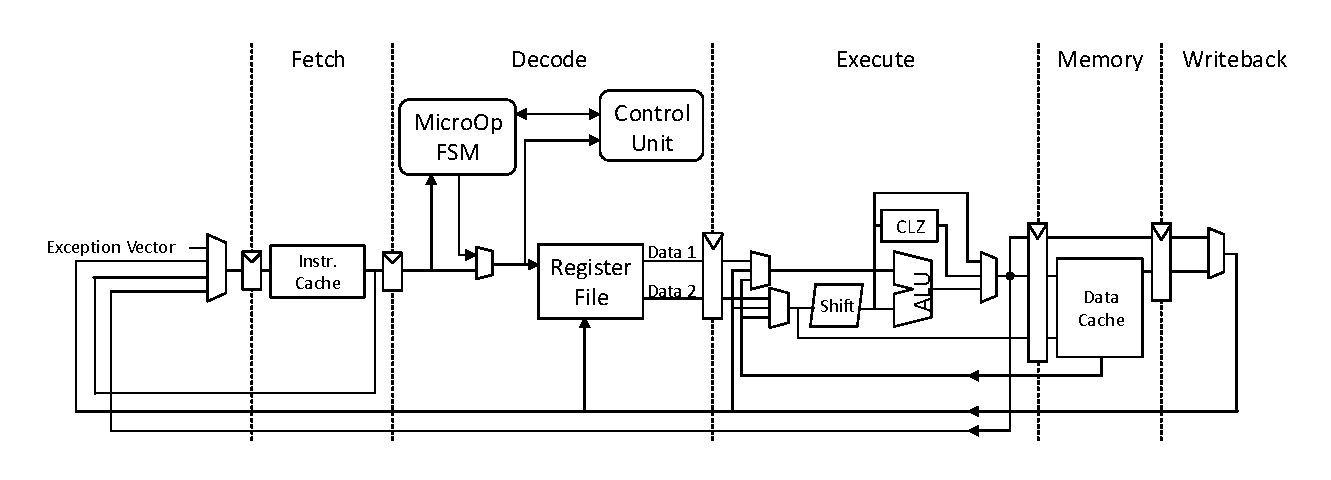
\includegraphics[width=\textwidth]{./diagrams/datapath_simple.pdf}
\caption{LEG processor core overview. More detailed diagrams are shown in the relevant sections below.}
\label{fig:core}
\end{figure}


LEG supports a subset of the ARMv5 instruction set. 
Known exceptions are the entire Thumb instruction set, LDM(2), and the rotate functionality of memory instructions.
The rotate functionality is not implemented because it appears to be unsupported in the version of qemu used to debug LEG.
All other addressing modes and instructions are supported, and any bugs that are discovered can be reported to the corresponding authors listed on the first page of this document.

The processor core is split into three main components.
The datapath contains the register file and hardware to execute arithmetic and memory operations, the controller sets multiplexers and other datapath control signals to create the specific behavior of each instruction, and the hazard unit detects dependencies between instructions and stalls the pipeline to resolve them.
A simplified overview of the processor core is summarized in Figure \ref{fig:core}.
More information about these subsystems can be found in later sections.
The datapath is described in Section \ref{sec:dp}, the controller in Section \ref{sec:c} and the hazard unit in Section \ref{sec:h}.

The full processor core diagram is shown in Figure \ref{fig:pipelinedfull} and is also included as a high quality PDF in the \texttt{documentation/diagrams} directory.

\begin{figure}[h!]
\centering
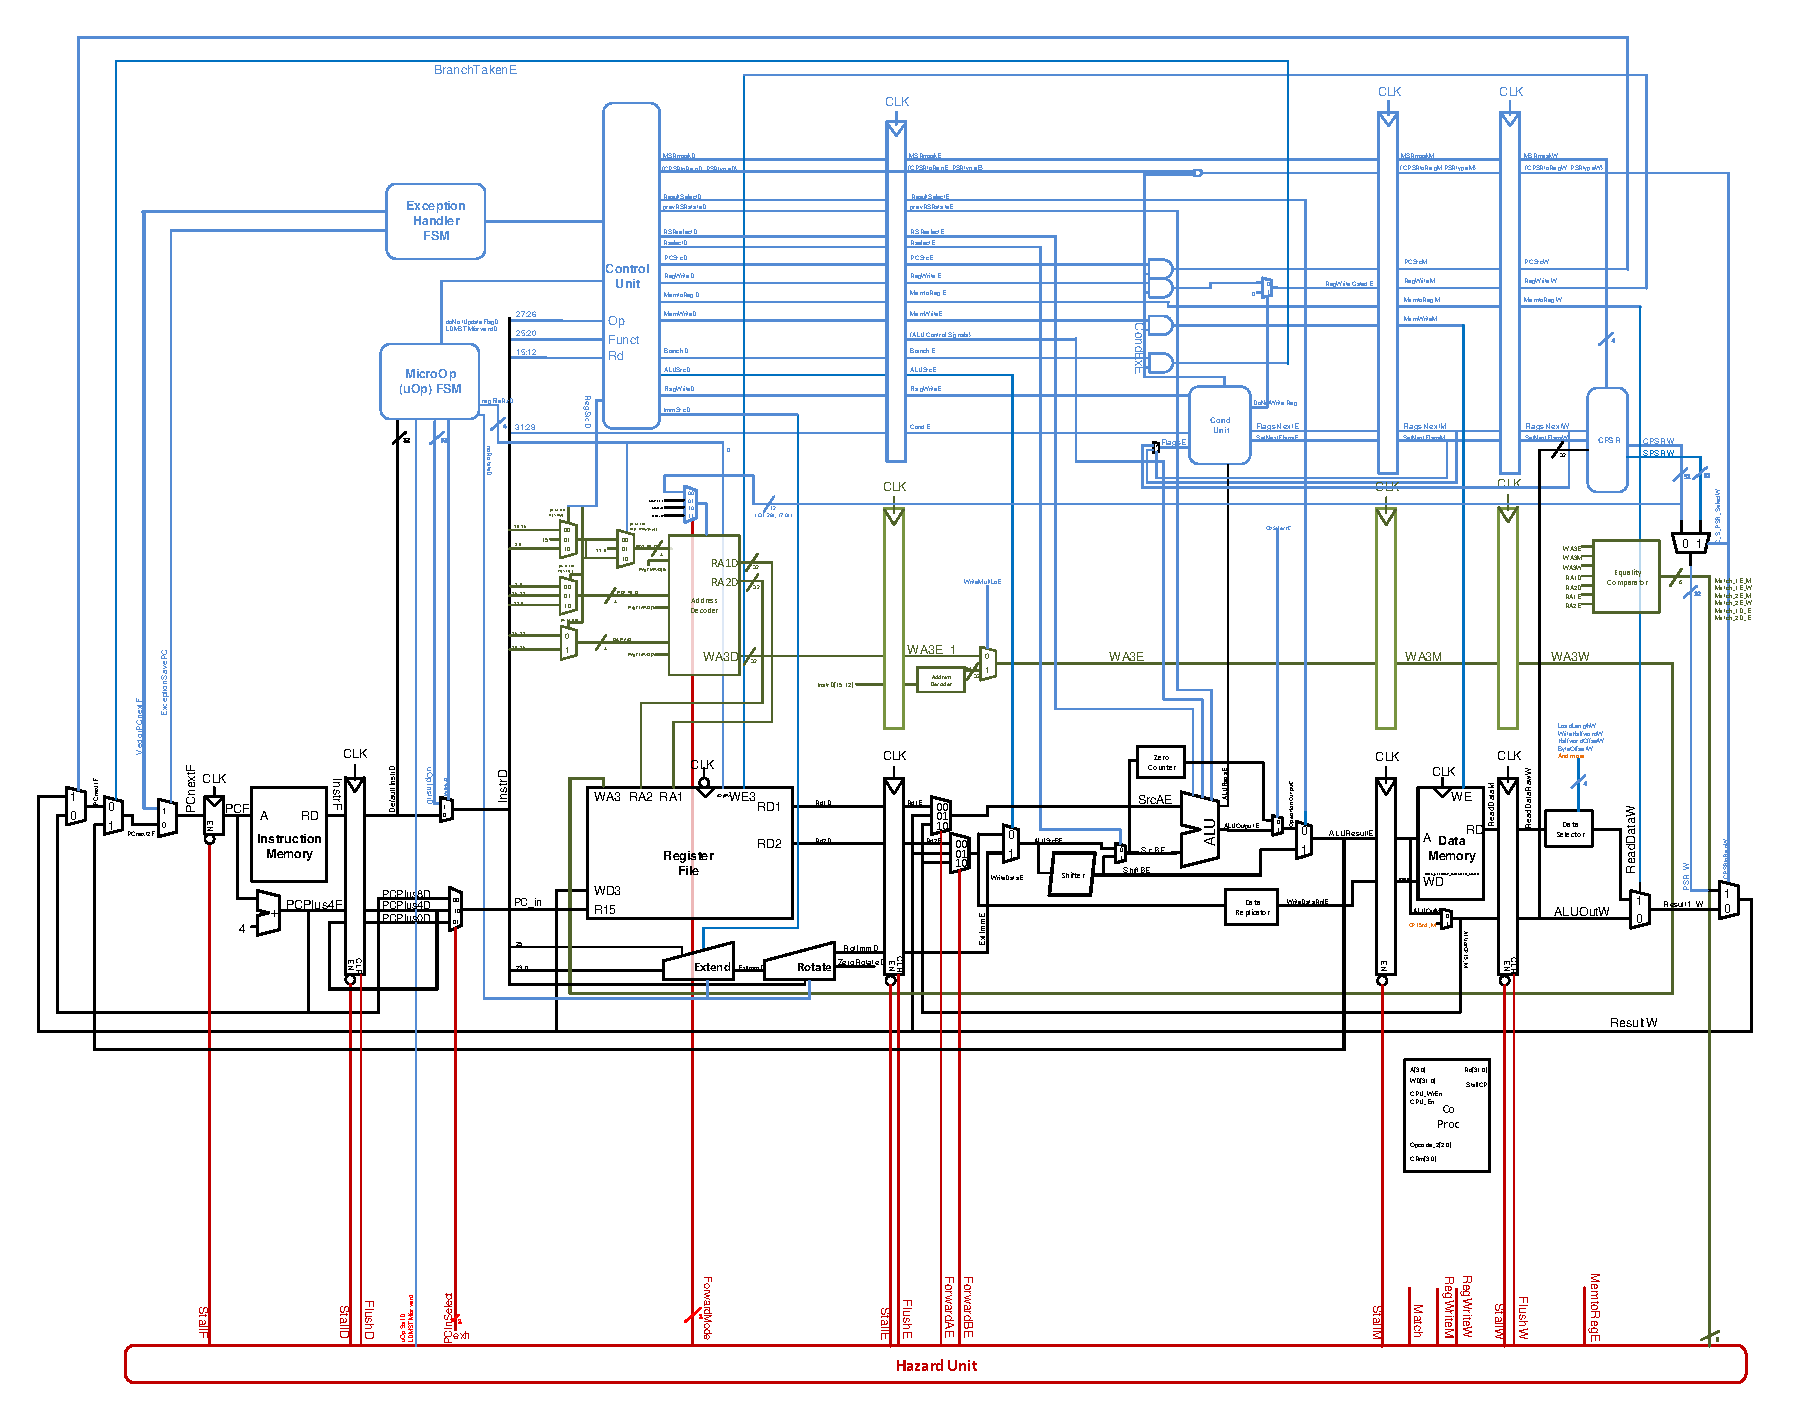
\includegraphics[width=\textwidth]{./diagrams/pipelinedfull.pdf}
\caption{LEG pipeline showing datapath (black), controller (blue), hazard unit (red), and a register file decoder also called the addresspath (green). A high resolution PDF is included in the diagrams directory.}
\label{fig:pipelinedfull}
\end{figure}

\subsection{Memory System}
The memory system includes L1 instruction and data
caches, a TLB, and corresponding address translation hardware shown in \ref{fig:mem}. The bus connecting the peripherals, translation hardware, and caches is compatible with the AHB-Lite protocol, but does not implement burst mode, protection control, or HRESP.
Descriptions of several of the caches can be found in sections \ref{sec:dcache} and \ref{sec:icache}.
%It is useful to track memory acesses for testing the debugging the memory system.
%If an error has occurred, then it is only detected once the incorrect value is read into a register.
%For this reason, debugging statements have been added to \texttt{testbench.sv} to allow memory access recording.

\begin{figure}[h!]
\centering
% TODO: update this with pdf image
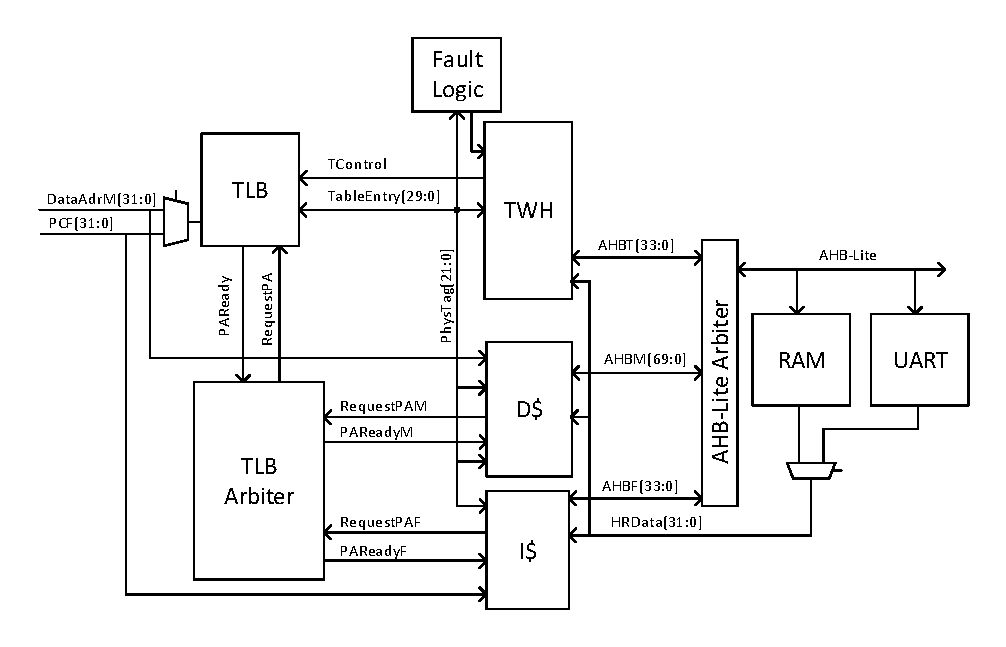
\includegraphics[width=\textwidth]{./diagrams/mmu.pdf}
\caption{Memory system including physically tagged caches, address translation hardware, and bus. The translation walk hardware (TWH), data and
instruction cache all desire access to the bus (right). The AHB-Arbiter
arbitrates bus control among those three modules. Instead of using two TLBS,
one for each cache, one (top left) is shared among the instruction cache and
data cache to conserve space. Similar to the AHB-Arbiter, the TLB arbiter
mediates control over the TLB request and ready signals.}
\label{fig:mem}
\end{figure}

\subsection{Exception and Interrupt Handler}

The LEG interrupt handler supports all exception types and privileged modes with the Base Restored Abort Model.
The interrupt handler is implemented as a finite state machine in \texttt{leg\_pipelined/exception\_handler.sv}.
This state machine stalls the correct pipeline stages and controls the datapath to branch to the corresponding exception vector.
More information about the exception handler can be found in Section \ref{sec:exh}


\section{Datapath}
\label{sec:dp}
This section gives an overview of the LEG datapath. 
The datapath is pipelined with five stages: Fetch, Decode, Execute, Memory, and Writeback. 
The stages can be flushed or stalled by the Hazard unit, and data flow is selected by the Controller module.

\noindent Datapath components are illustrated in black on the processor diagram \\\texttt{documentation/diagrams/pipelinedfull.pdf}

\subsection{Relevant Files}

\begin{tabular}{|l|p{120mm}|}
\hline \textbf{File}  & \textbf{Description} \\ 
\hline datapath.sv & Contains all datapath logic and signals for the LEG processor.  \\ 
\hline adder.sv & A parameterized adder. \\ 
\hline addressdecode.sv & Decodes a 4 bit register number and the current processor mode to a one-hot register file select signal. \\ 
\hline regfile.sv & A 32 entry by 32 bit register file containing the 31 general purpose registers and one scratch register for micro operations. Located in the Decode stage. \\ 
\hline extend.sv & Handles extending immediate values of varying width to 32 bits. Located in the Decode stage. \\ 
\hline rotator.sv & A funnel shifter that rotates the 32 bit immediate in data processing instructions. Located in the Decode stage. \\ 
\hline barrel\_shifter.sv & An efficient two stage logarithmic barrel shifter that implements LSR, ASR, LSL, ROR, and RRX shift types. Located in the Execute stage. \\ 
\hline alu.sv & Arithmetic Logic Unit that computes and selects between addition, AND, OR, and XOR operations. Located in the Execute stage. \\ 
\hline zero\_counter.sv & Outputs the number of leading zeros in its input. This module is a good target for optimization in class projects. Located in Execute stage. \\ 
\hline data\_replicator.sv & Selects the size of data required for a memory operation and replicates it to fill the available byte positions. Located in Execute stage. \\ 
\hline data\_selector.sv & Masks data words read from memory and extends them to 32 bits. Located in Writeback stage. \\ 
\hline 
\end{tabular} 

\subsection{Fetch Stage}
The Fetch stage reads an instruction from instruction memory using the register 15, the program counter (PC).
This PC is selected from several sources based on branch or exception status.
The instruction memory is shown in the datapath in the processor diagram, but is actually implemented externally to the processor core. 
See Section \ref{sec:i-cache} for more information.

\subsection{Decode Stage}
In the Decode stage registers are read and immediates are extended and rotated to the form required for arithmetic processing. 
Note that the instruction processed in the decode stage may not match the instruction read in the execute stage due to micro operation decoding (see Section \ref{sec:uop}).

\subsection{Execute Stage}
The Execute stage processes instruction operands into a resultant value. 
First forwarded register values are optionally selected based on signals from the Hazard unit (Section \ref{sec:fwd}).
Shifts or rotates are applied to the second operand and results are computed by the zero counter and ALU. 
The second operand is also processed as data for a potential memory operation. 
Finally, the output is selected from the correct functional unit based on the instruction type.

\subsection{Memory Stage}
The values computed in the Execute stage may be used as data and address in the Memory stage.
The result may also bypass the data memory when a store operation is not performed.
As with the instruction memory, the data memory is drawn in the datapath but is actually a separate functional unit described in Section \ref{sec:d-cache}.

\subsection{Writeback Stage}
In the Writeback stage the result of the Memory stage is fed back to be written to registers or the PC.


\section{Controller}
\label{sec:c}
The LEG controller maintains the flags and status register and handles control flow of the datapath.
The controller has the same pipeline stages as the datapath, but most signals are generated in the Decode stage. 
These signals then advance through the processor in step with the corresponding instruction.

\subsection{Relevant Files}
\begin{tabular}{|l|p{120mm}|}
\hline \textbf{File}  & \textbf{Description} \\ 
\hline controller.sv & Contains instruction decode logic to control datapath flow. Also includes micro operation state machine, exception handler, and program status registers.\\ 
\hline micropsfsm.sv & Mealy finite state machine that decodes complex instructions into sequences of simpler instructions. The instruction output by this module is used in the remaining controller decode logic.\\ 
\hline shift\_control.sv & Selects shift types, decodes shift amount, and determines shifter carry out from datapath barrel shifter. \\ 
\hline alu\_decoder.sv & Generates control signals for the ALU operation, inputs, and flags.\\
\hline memory\_mask.sv & Generates memory mask for storing different subsets of complete data words. \\
\hline conditional.sv & Checks conditional execution and kills writeback signals if an instruction should not be executed. Also generates the resultant flags of an instruction.\\
\hline exception\_handler.sv & A Mealy state machine that choreographs stalls, flushes, and branching when interrupts or exceptions are detected.\\
\hline cpsr.sv & Contains current and saved program status registers. Handles flag updates and verifies mode changes. \\
\hline 
\end{tabular} 


\subsection{Pipeline stages}
The controller Decode stage receives an instruction from the micro op FSM and generates datapath control signals.
Many control signals are needed for the execute, memory, and writeback stages. 
These are pipelined to follow the corresponding instruction, including any flushes or stalls.

Conditional execution is checked in the Execute stage.
If an instruction fails the condition check it continues to propagate through the datapath but all writeback and forwarding signals are killed. 
Thus the instruction has no effect on processor state.

\subsection{CPSR and Flags}
After a CPSR update the new flags and mode bits are forwarded to the next instruction before propagating to the writeback stage. 
The pipeline is also stalled as necessary so that the correct registers are read after any mode change.
This ensures correct operation of conditional and privileged instructions.

\subsection{MicroOp State Machine}\label{sec:uop}

The micro operation state machine is responsible for decoding complex instructions into sequences of simpler instructions. 
It takes the fetched instruction as input and outputs the instruction that is used in the rest of the processor logic. 
Additionally, the state machine outputs extra signals to enable special functionality of some instructions, such as preserving a carry bit from a previous micro op stage. 
The state transition diagram and instruction outputs of the micro op state machine is shown in Figure \ref{fig:uopdiagram}.
Table \ref{table:uops} lists the number of instructions issued for most micro operations.

\begin{figure}[h!]
\centering
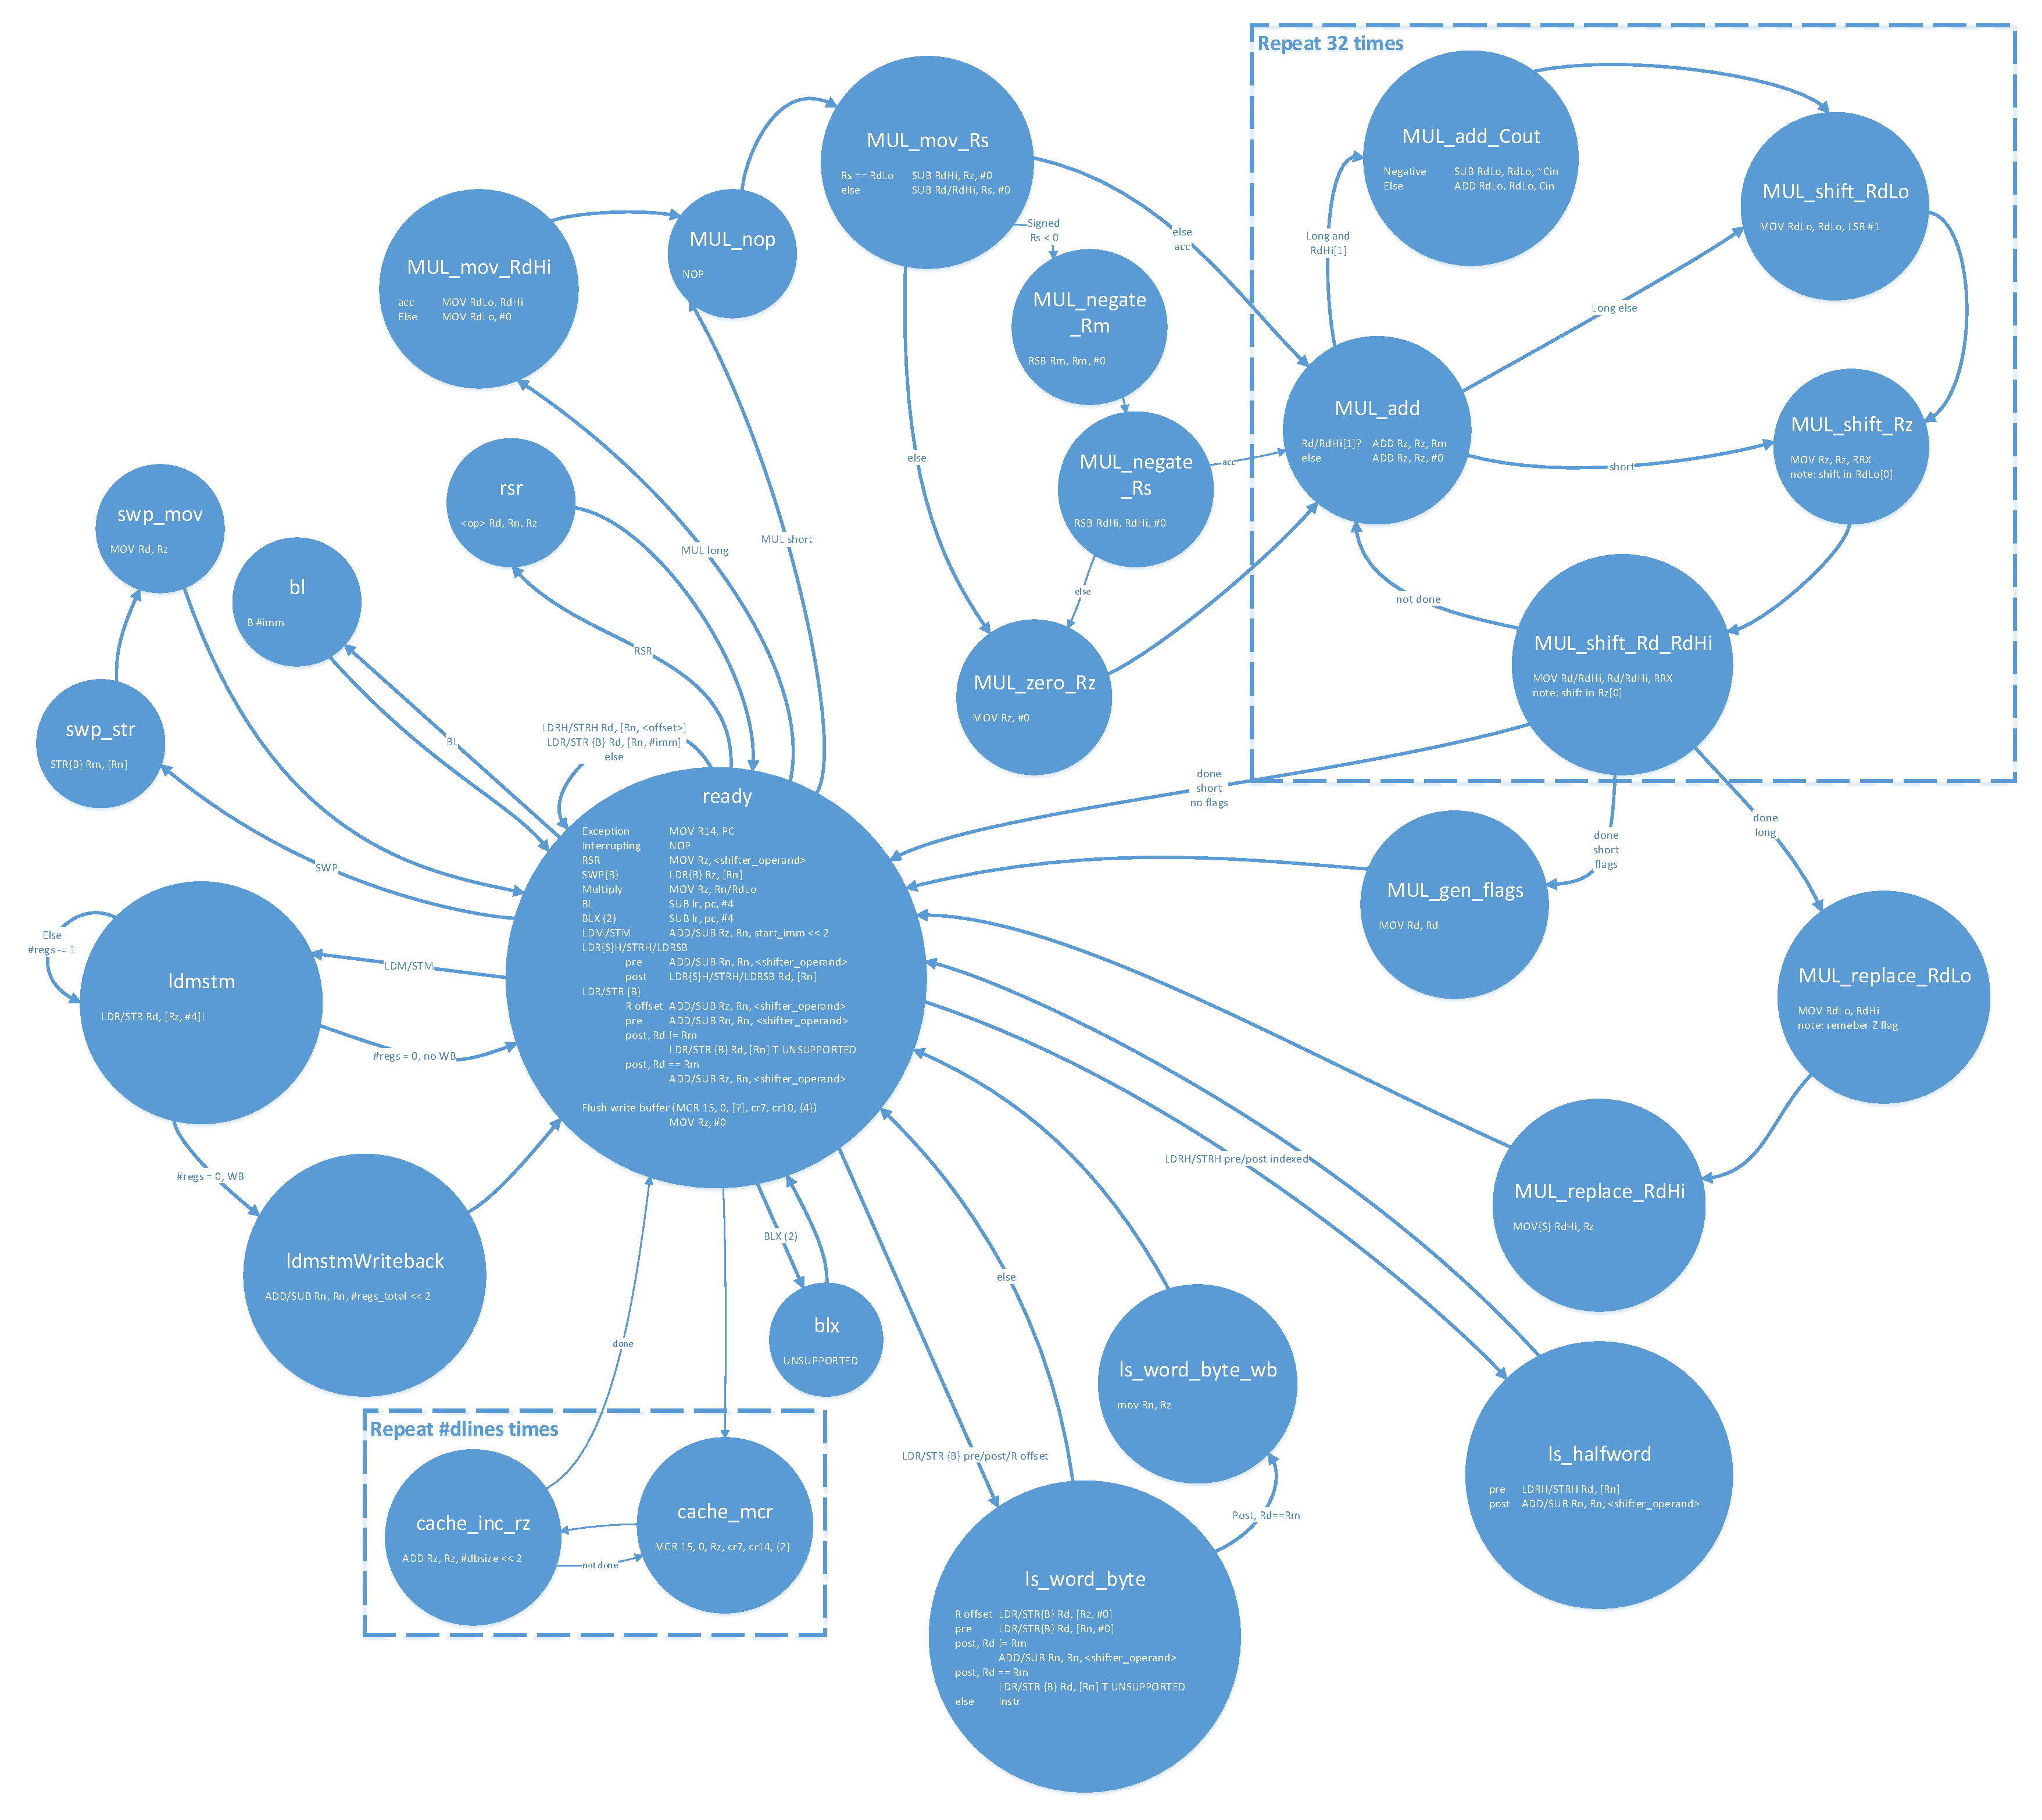
\includegraphics[width=\textwidth]{./diagrams/micropfsm_drawing.pdf}
\caption{State transition diagram for the micro op state machine. A high quality PDF is available as \texttt{documentation/diagrams/micropfsm\_drawing}}
\label{fig:uopdiagram}
\end{figure}

\begin{table}[h!]
\centering
\begin{tabular}{|l|l|}
\hline
\textbf{Instruction} & \textbf{Operations}\\
\hline
Exception & 1\\
\hline
Write buffer flush & 2 x \#dlines + 1\\
\hline
LDRH / STRH & 1-2\\
\hline
LDR / LDRB / STR / STRB & 1-3\\
\hline
Register shifted register & 2\\
\hline
BL / BLX & 2\\
\hline
SWP / SWPB & 3\\
\hline
LDM / STM & 2-18\\
\hline
MUL / MLA & 98-100\\
\hline
UMULL / UMLAL & 133-166\\
\hline
SMULL / SMLAL & 135-168\\
\hline
\end{tabular}
\caption{Number of micro-operations corresponding to each complex instruction}
\label{table:uops}
\end{table}



\subsection{Exception Issue State Machine}

The LEG exception handler is implemented as a state machine that allows interrupts and exceptions to be prioritized. 
When exceptions are detected the state machine allows the instructions before the exception-generating instruction to finish propagating through the pipeline but blocks any further instructions. 
Once the final pre-exception instruction has completed Writeback the state machine triggers saving of the program counter, mode switching, and branching to the configured exception vector.
This delay is necessary because pre-exception instructions may change the processor state including the behavior of the exception.


\section{Hazard Unit}
\label{sec:h}
The Hazard unit detects potential conflicts between pipeline stages and stalls, flushes, or forwards values between stages to resolve them.

\subsection{Relevant Files}
\begin{tabular}{|l|p{120mm}|}
\hline \textbf{File}  & \textbf{Description} \\ 
\hline hazard.sv & Generates flush, stall, and forward signals for the datapath and controller based on instruction types and processor state. \\
\hline eqcmp.sv & Compares register numbers at different pipeline stages to inform forward signals. \\
\hline 
\end{tabular} 

\subsection{Stalls}
All pipeline stages can be stalled, but the Execute, Memory, and Decode stages are stalled only because of data and instruction cache behavior.
The Fetch stage is additionally stalled during micro ops, coprocessor and CPSR operations, PC writes.
The Decode stage can be stalled for micro ops and by the exception handler.

Both Fetch and Decode are stalled during a read after write (RAW) hazard when a register is loaded from memory. 
Other RAW hazards are handled by forwarding.

\subsection{Flushes}
Various pipeline stages are flushed in the same circumstances as they are stalled. 
This behavior kills writeback signals during stalls so actions are not performed multiple times.
Additional flushes take place whenever a branch is taken since LEG does not implement branch prediction.

\subsection{Forwarding}\label{sec:fwd}
Read after write (RAW) hazards occur when a register that is written by one instruction is read by a later instruction before the change has propagated through to the Writeback stage.
Most RAW hazards can be solved by forwarding values from the Memory or Writeback stages to the Execute stage rather than stalling.
These hazards are detected by comparing the register number being used as an operand in each stage and then selecting the appropriate value to forward. 
This forwarding is gated by the corresponding stage's register writeback signal so values from unexecuted or flushed instructions are not used.

%\section{Exception Handler}
%\input{tex/exh.tex}

\section{Data Cache} \label{sec:dcache}
The data cache is a writeback, 2 way associative cache. 
Figure \ref{fig:dcachediag} includes a diagram of the data cache.
The cache uses physical tagging and virtual indexing, so the number of bytes in each way is limited to the size of a tiny translation page (1024 bytes). 
The default cache size is $64 \text{ lines} \cdot 4 \text{ words/line} \cdot 4 \text{ bytes/word} = 1024 \text{ bytes}$. 
The number of lines per way is parameterized, and the replacement policy implemented is Least Recently Used (LRU).

	\begin{figure}
	\centering
	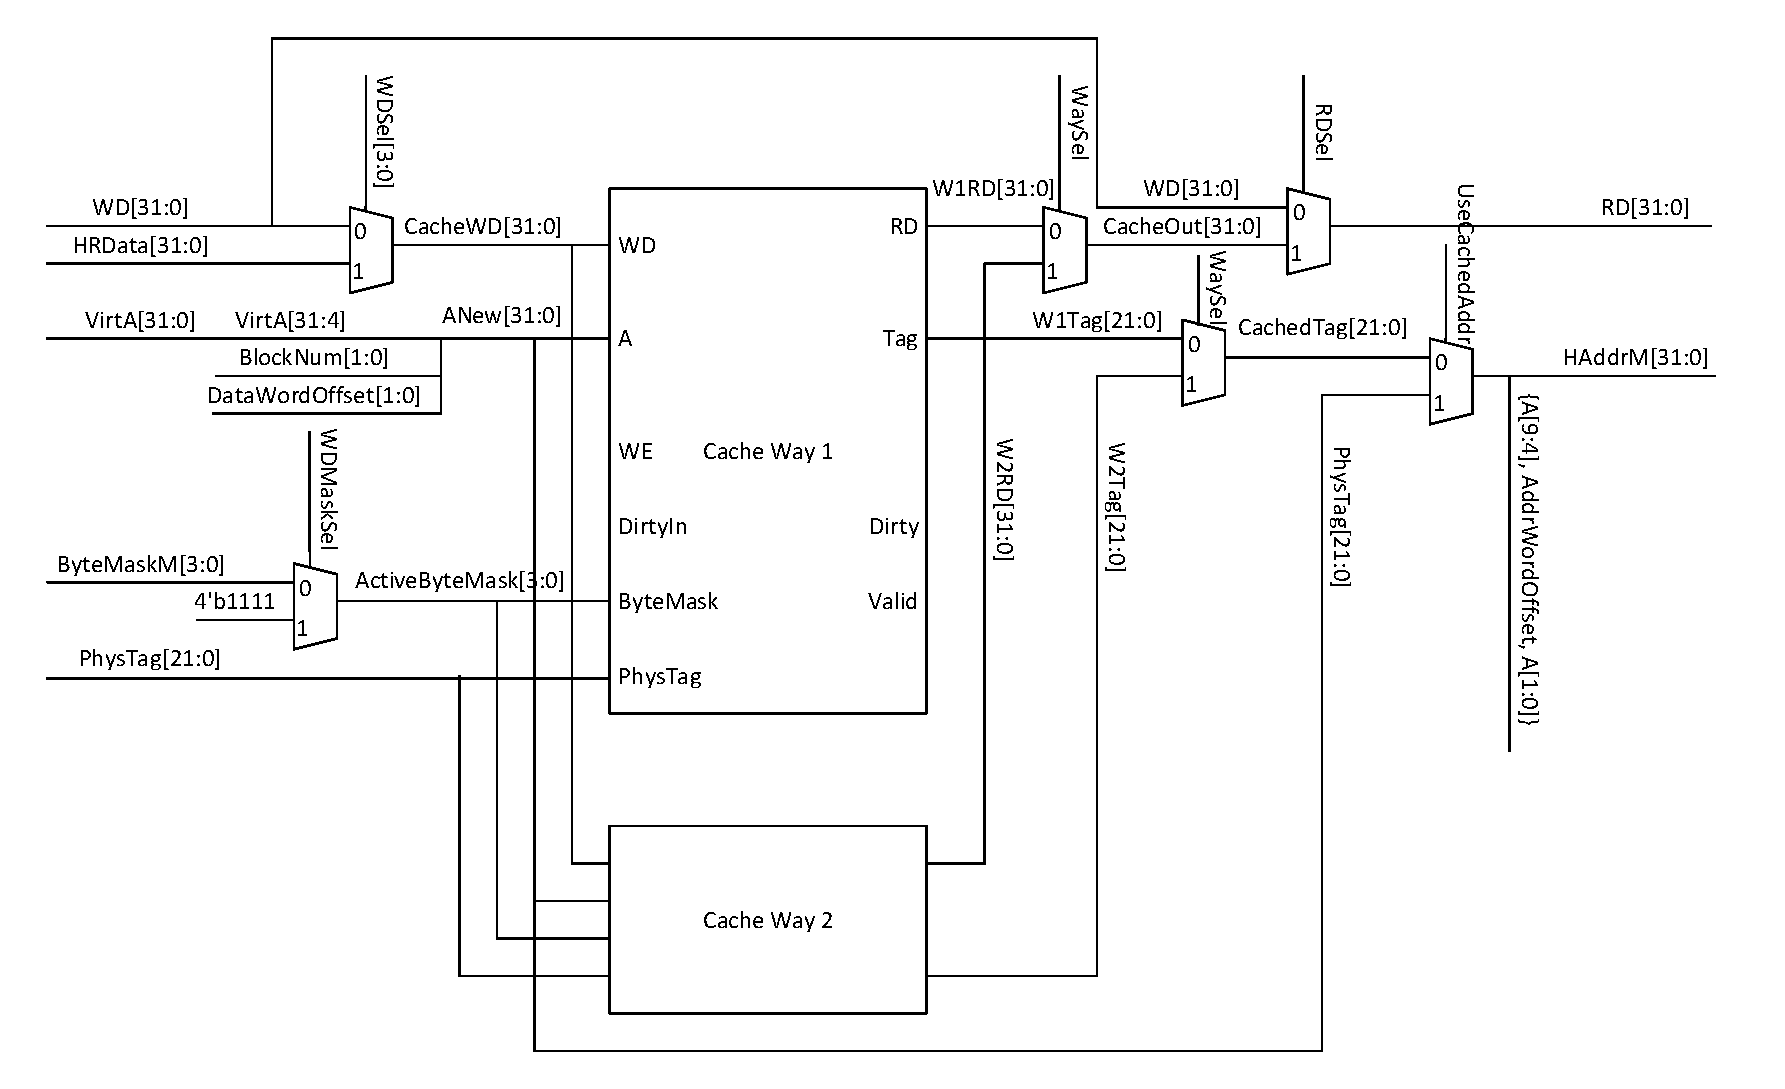
\includegraphics[width=\textwidth]{diagrams/data_cache.pdf}
	\caption{Diagram of 2 way set associative data cache. Note that many of the control signals are not shown in this diagram for simplicity. Also, the second cache way is identical to the first.}
	\label{fig:dcachediag}
	\end{figure}

\subsection{Relevant Files}

	Table \ref{table:drel} shows the files that are used by the data cache and Table \ref{table:dio} lists the top level inputs and outputs.

	\begin{table}
	\begin{tabular}{|l|p{70mm}|}
	\hline File  & Description \\ 
	\hline  data\_writeback\_associative\_cache.sv & Top level D\$ module \\ 
	\hline  data\_writeback\_controller.sv & Controller logic for the D\$.
	Contains the primary state machine described in section \ref{sec:dstate} \\ 
	\hline  data\_writeback\_associative\_memory.sv & 
	Memory module containing the both cache ways, the LRU memory, and way selection mux's.
	This module is used in both the instruction and data caches.
	The instruction cache fixes the dirty and clean inputs to zero, because it is a read only cache.\\ 
	\hline  data\_writeback\_associative\_cache\_way.sv & 
	Contains the memory associated with one cache way. This includes four words per line along with the valid, dirty, and tag bits. \\ 
	\hline  word\_memory.sv & Byte addressable word memory  \\
	\hline
	\end{tabular} 
	\caption{Data cache files}
	\label{table:drel}
	\end{table}

	\begin{table}
	\begin{tabular}{|l|p{85mm}|l|}
	\hline Port & Description & I/O \\ 
	\hline clk & Clock input &  I \\ 
	\hline reset & Global reset signal &  I \\ 
	\hline MemWriteM & Write signal from datapath &  I \\ 
	\hline MemtoRegM & Read signal from datapah & I \\ 
	\hline IStall & Instruction cache stall. Used to avoid multiple data acesses for the same instruction & I \\
	\hline VirtA[31:0] & Virtual address from the leg datapath & I \\
	\hline WD[31:0] & Write data from LEG datapath & I \\
	\hline CP15en & Enable signal from the coprocessor & I \\
	\hline Inv & Invalidate line signal from the coprocessor & I \\
	\hline AddrOp & Indicates coprocessor is invalidating or cleaning using a virtual address instead of a set index. When high, only clean or invalidate on a hit in the data cache.& I \\
	\hline InvAllMid & When InvAllMid and Inv are high, invalidate all lines from cache. This signal is driven by the coprocessor & I \\
	\hline CurrCBit & Cachable bit for the current TLB entry & I \\
	\hline PAReady & Indicates TLB entry is valid for the data cache. The data cache uses the physical address and control bits from the TLB & I \\
	\hline PhysTag[tbits-1:0] & Physical Tag from the TLB & I \\
	\hline ByteMaskM[3:0] & ByteMask from leg controller & I \\
	\hline HRData[31:0] & Data from the AHB Bus & I \\
	\hline BusReady & AHB Ready signal & I \\
	\hline MSel & Indicates data cache has control of the AHB Bus & I \\
	\hline Stall & Stall signal from the data cache controller & O \\
	\hline RequestPA & Request a physical address from the TLB & O \\
	\hline HWData[31:0] & AHB Write data & O \\
	\hline RD[31:0] & Data output from the cache. This is the same as HWData. & O \\
	\hline HAddr[31:0] & AHB write address & O \\
	\hline HSizeM & AHB write size & O \\
	\hline HRequestM & Request AHB control & O \\
	\hline HWriteM & AHB write enable & O \\
	\hline
	\end{tabular} 
	\caption{Data cache I/O (data\_writeback\_associative\_cache.sv)}
	\label{table:dio}
	\end{table}
	% TODO: Fix the label and reference

\subsection{Data Cache States}
\label{sec:dstate}

Below is an explanation of the data cache states.

\begin{enumerate}
	\item READY 
	The ready state is the default state for the data cache.
	Upon a cache hit, the data cache will remain in the READY state.

	\item WRITEBACK
	The cache enters the writeback state to writeback each word from the line to memory.
	If the data cache attempts to replace a dirty line, then it is written back first.
	The data cache stays in this state for at least three cycles to writeback the first three words from the dirty line.

	\item LASTWRITEBACK:
	The last writeback state in the cache. 
	During this state, the data cache does not request a new memory access.
	It waits for the last writeback to complete.

	\item MEMREAD:
	Data cache enters this state on a cache miss to read data from memory.
	The cache reads four words sequentiall from the AHB Bus.

	\item LASTREAD:
	The last memread state in the cache. 
	During this state, the data cache does not request a new memory access.
	It waits for the last memory read to complete.

	\item NEXTINSTR:
	The next instr state removes the stall on the pipeline and allows the instructions to move one stage down the pipeline. If this stage did not exist, then the instruction at the data stage would remain the same and after the requested data is retrieved, the same data would be retrieved again. 

	\item WAIT:
	The data cache enters this state when simultaneous data and instruction stalls occur. 
	The data cache has bus precedence, so after it is done using the bus it waits for the instruction cache to retrieve data before handling the next request. 
	This state avoids repeating data acesses when the processor stalls.

	\item DWRITE:
	This state handles disables full word writes to main memory.
	
\end{enumerate}

\pagebreak

\section{Instruction Cache} \label{sec:icache}
The instruction cache is a read only, 2 way associative cache. 
The instruction cache uses physical tagging and virtual indexing, so the number of bytes in each way is limited to the size of a tiny translation page (1024 bytes). 
The default cache size is $64 \text{ lines} \cdot 4 \text{ words/line} \cdot 4 \text{ bytes/word} = 1024 \text{ bytes}$. 
The number of lines per way is parameterized, and the replacement policy implemented is Least Recently Used (LRU).
The instruction cache uses the same memory modules as the data cache, but disables the dirty and clean signal.
The controller logic is much simpler for the instruction cache, because it is read only.
	% TODO: Get a diagram of the instruction cache
%	Figure \ref{fig:icachediag} includes a diagram of the instruction cache.
%	See the code for more information.
%	\begin{figure} \label{fig:icachediag}
%	\centering
%	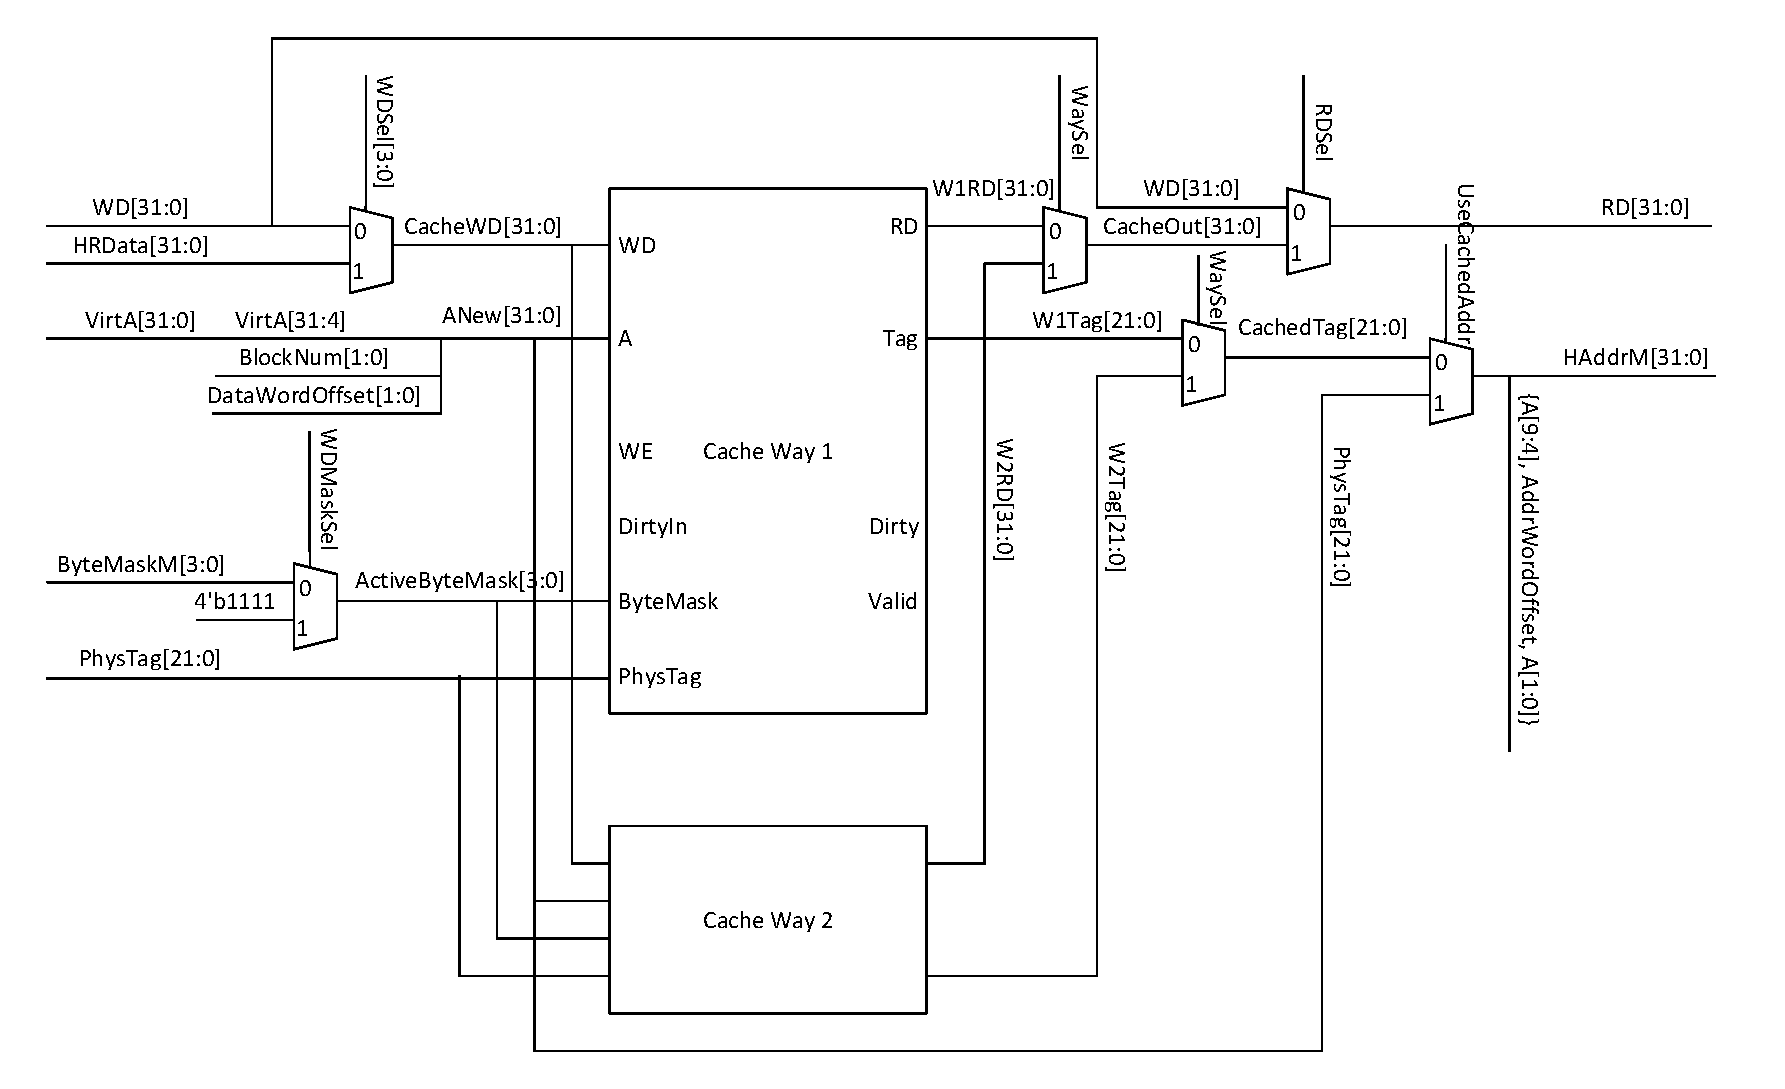
\includegraphics[width=\textwidth]{diagrams/data_cache.pdf}
%	\caption{Diagram of 2 way set associative instruction cache. Controller logic in blue}
%	\end{figure}

\subsection{Relevant Files}

	Table \ref{table:irel} shows the files that are used by the instruction cache and Table \ref{table:instrio} lists the top level inputs and outputs.

	\begin{table} \label{table:irel}
	\begin{tabular}{|l|p{70mm}|}
	\hline File  & Description \\ 
	\hline  instr\_cache.sv & Top level I\$ module \\ 
	\hline  instr\_cache\_controller.sv & Controller logic for the I\$.
	Contains the primary state machine described in section \ref{sec:istate} \\ 
	\hline  data\_writeback\_associative\_memory.sv & 
	Memory module containing the both cache ways, the LRU memory, and way selection mux's.
	This module is used in both the instruction and data caches.
	The instruction cache fixes the dirty and clean inputs to zero, because it is a read only cache.\\ 
	\hline  data\_writeback\_associative\_cache\_way.sv & 
	Contains the memory associated with one cache way. This includes four words per line along with the valid, and tag bits. \\ 
	\hline  word\_memory.sv & Byte addressable word memory  \\
	\hline
	\end{tabular} 
	\caption{Instruction cache files}
	\end{table}

	\begin{table} \label{table:instrio}
	\begin{tabular}{|l|p{85mm}|l|}
	\hline Port & Description & I/O \\ 
	\hline clk & Clock input &  I \\ 
	\hline reset & Global reset signal &  I \\ 
	\hline uOpStallD & Micro-Op stall signal. This signal is used to prevent repeated memory assesses when the pipeline is stalled &  I \\ 
	\hline A[31:0] & Virtual address from the leg datapath & I \\
	\hline CP15en & Enable signal from the coprocessor & I \\
	\hline AddrOp & Indicates coprocessor is invalidating using a virtual address instead of a set index. When high, only invalidate on a hit in the instruction cache.& I \\
	\hline InvAllMid & When InvAllMid and Inv are high, invalidate all lines from cache. This signal is driven by the coprocessor & I \\
	\hline Inv & Invalidate signal from the coprocessor & I \\
	% \hline CurrCBit & Cachable bit for the current TLB entry & I \\
	\hline PhysTag[tbits-1:0] & Physical Tag from the TLB & I \\
	\hline PAReadyF & Indicates TLB entry is valid for the instruction cache. The instruction cache uses the physical address and control bits from the TLB & I \\
	\hline FSel & Indicates instruction cache has control of the AHB Bus & I \\
	\hline BusReady & AHB Ready signal & I \\
	\hline HRData[31:0] & Data from the AHB Bus & I \\
	\hline RD[31:0] & Data output from the cache. This is the same as HWData. & O \\
	\hline IStall & IStall signal from the instruction cache controller & O \\
	\hline HRequestF & Request AHB control & O \\
	\hline HAddrF[31:0] & AHB address & O \\
	\hline RequestPA & Request a physical address from the TLB & O \\
	\hline
	\end{tabular} 
	\caption{Instruction cache I/O (instr\_cache.sv)}
	\end{table}
	% TODO: fix the label and reference

\subsection{Instruction Cache States}
\label{sec:istate}

Below is an explanation of the instruction cache states.

\begin{enumerate}
	\item READY 
	The ready state is the default state for the instruction cache.
	Upon a cache hit, the instruction cache will remain in the READY state.

	\item MEMREAD:
	Instruction cache enters this state on a cache miss to read data from memory.
	The cache reads four words sequentially from the AHB Bus.

	\item LASTREAD:
	The last memread state in the cache. 
	During this state, the instruction cache does not request a new memory access.
	It waits for the last memory read to complete.

	\item NEXTINSTR:
	The next instr state removes the stall on the pipeline and allows the instructions to move one stage down the pipeline. If this stage did not exist, then the instruction at the fetch stage would remain the same and after the requested instruction is retrieved, the same data would be retrieved again. 

\end{enumerate}

\pagebreak


\end{document}
